%txs:///pdflatex | txs:///bibtex | txs:///nomenclature | txs:///pdflatex | txs:///pdflatex | txs:///drivebackup | txs:///cleanup

\documentclass[10pt,a4paper]{article}

%\usepackage[off,crop={off},runs={2}]{auto-pst-pdf}
\usepackage[crop={on},runs={2}]{auto-pst-pdf}

\usepackage{preamble}
\usepackage{import}
\graphicspath{{./figs/}{./figs/eps_manual/}{./figs/eps/}{./figs/nmrs/}}

\begin{document}

\section*{The synthesis and biological evaluation of a library of autoinducer-antibiotic conjugates - Lois Overvoorde}

Bacterial resistance to antibiotics is a serious global health threat, and new, safe and effective antibiotics are required urgently. A new class of antibiotic, namely sideophore-antibiotic conjugates, has shown promise in initial studies. Siderophores are used by bacteria for iron uptake, and so attaching antibiotics to them allows the antibiotic to be carried across cell membranes. We have designed conjugates using a similar approach, but using bacterial autoinducers instead of siderophores. Autoinducers are required for coordination of bacterial behaviours and are involved in the control of swarming, virulence factor production and biofilm formation. 

The library was synthesised in two halves which were then coupled together using either a copper(I)-catalysed azide-alkyne cycloaddition or peptide coupling. It was decided to focus on the autoinducers produced by \textit{Pseudomonas aeruginosa} as it is a significant human pathogen which displays high resistance to many antibiotics and uses quorum sensing to coordinate its group behaviours.
Several conjugates of  C$_4$-HSL derivatives were also included, as a thiolactone-antibiotic conjugate has been shown to possess increased activity against established biofilms compared with the unmodified antibiotic.
Autoinducer derivatives were coupled with derivatives of ciprofloxacin or trimethoprim. It is hoped that the autoinducers will deliver the attached antibiotic into the cell, thus potentially increasing its potency or even restoring its efficacy against resistant strains.

Biological testing of the conjugates is in progress, and results will be included in the final thesis.
	
\begin{scheme}[H]
	\begin{center}
		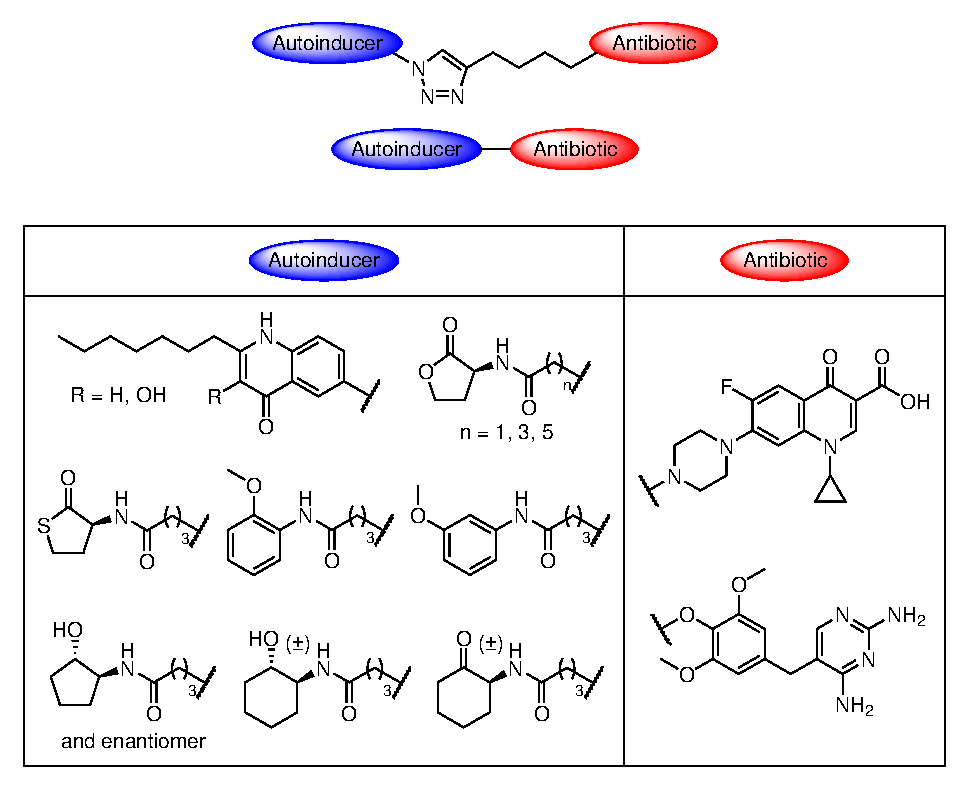
\includegraphics[width=\linewidth]{Summary_1}
		%\caption{}
	\end{center}
\end{scheme}

\end{document}